\documentclass{article}
\usepackage{ctex}
\usepackage{graphicx}
\usepackage{amsmath}
\usepackage{indentfirst}
\usepackage{titlesec}
\usepackage{setspace}
\usepackage{subfigure}
\usepackage{caption}
\usepackage{float}
\usepackage{booktabs}
\usepackage{geometry}
\usepackage{multirow}
\usepackage{hyperref}
\geometry{left=1.2cm,right=1.2cm,top=2cm,bottom=2cm}
\title{\songti \zihao{2}\bfseries HW4第9题中心极限定理验证}
\titleformat*{\section}{\songti\zihao{4}\bfseries}
\titleformat*{\subsection}{\songti\zihao{5}\bfseries}
\renewcommand\thesection{\arabic{section}}
\author{王启骅 PB20020580}
\begin{document}
	\maketitle
	\section{题目}
考虑泊松分布、指数分布,并再自设若干个随机分布(它们有相同或不同
的  $ \mu,\sigma $),通过Monte Carlo模拟,验证中心极限定理成立(N =2、5、10)。
	
	\section{算法原理}
泊松分布,首先产生满足泊松分布的随机数,根据泊松实验,对于一个[0,1]均匀随机数列u,计算该数列依次相乘,当刚好乘积小于$ e^{-\lambda} $时,返回上一个所乘的次数k即为满足泊松分布$ p(k)=\frac{\lambda^x}{x!}e^{-\lambda} $的随机数。对于该泊松分布$ \mu=\lambda $。


指数分布,对于一个[0,1]均匀随机数列u,根据直接抽样法,$ x=-\mu\ln(1-u) $,由于均匀分布u等效于$ x=-\mu\ln(u) $,即为$ p(x)=\frac{1}{\mu}\exp(-\frac{x}{\mu}) $的抽样。对于该指数分布$ \mu=\mu $。


均匀分布,在直接以[0,1]均匀随机数列u作为分布计算。对于该均匀分布$ \mu=0.5 $。


最后取高斯分布,根据Box-Muller法,对于[0,1]均匀随机数列u,v,抽样方法为$ x=\sqrt{-2\ln(u)}\cos(2\pi v) $。对于高斯分布$ \mu=0 $。
	\section{结果}
	这里取总点数k=$ 10^5 $,泊松分布$ \lambda=5 $,指数分布$ \mu=5 $,均匀分布位于[0,1]。绘制出了$ \frac{\langle f\rangle-\mu}{\sigma_f/\sqrt{N}} $的分布函数图
	\begin{figure}[!h]
		\centering
		\subfigure[N=2]{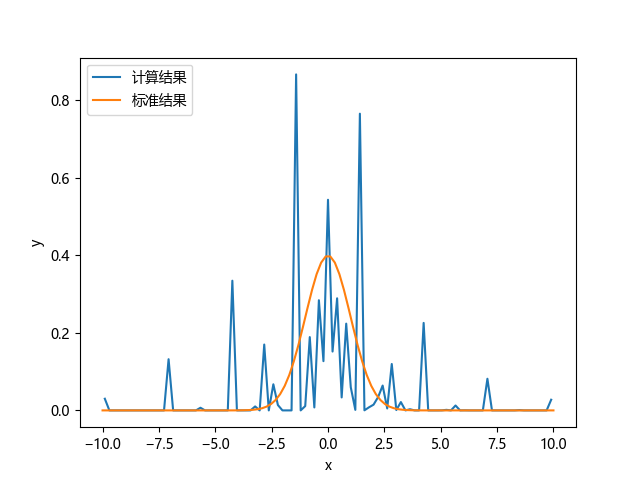
\includegraphics[scale=0.5]{poisson_2}}
		\subfigure[N=5]{	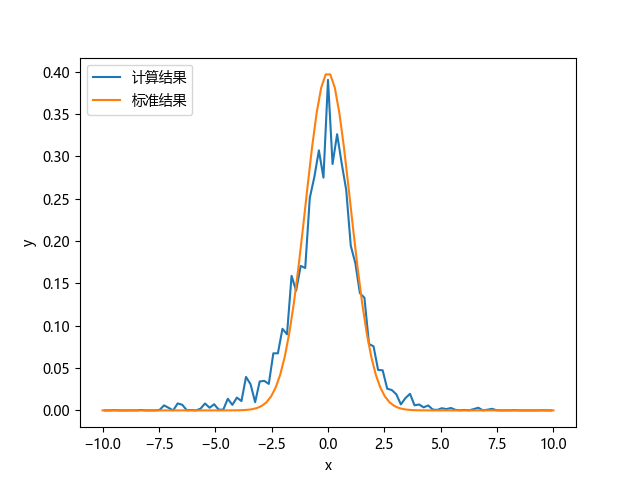
\includegraphics[scale=0.5]{poisson_5}}
		\subfigure[N=10]{	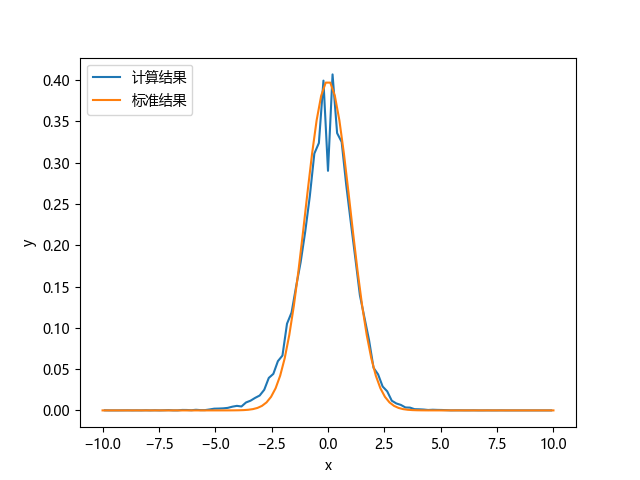
\includegraphics[scale=0.5]{poisson_10}}
		\captionsetup{font={small},labelfont=bf}
		\caption{\heiti\zihao{-5}Poisson}
		
	\end{figure}
	\begin{figure}[!h]
	\centering
	\subfigure[N=2]{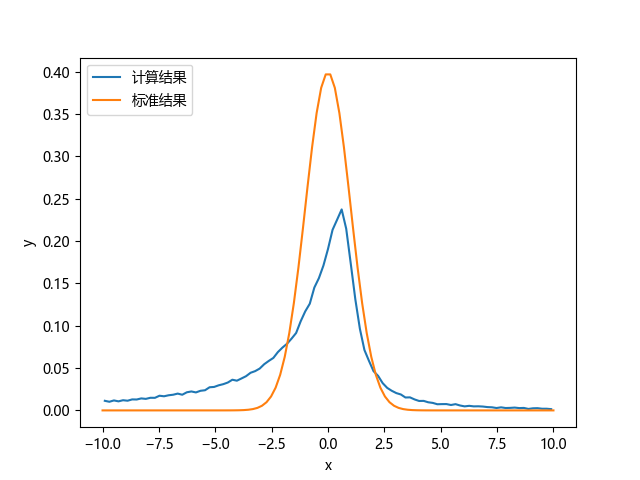
\includegraphics[scale=0.5]{exp_2}}
	\subfigure[N=5]{	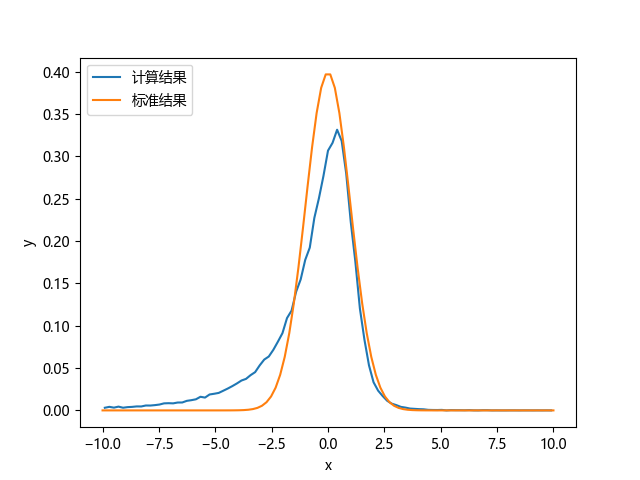
\includegraphics[scale=0.5]{exp_5}}
	\subfigure[N=10]{	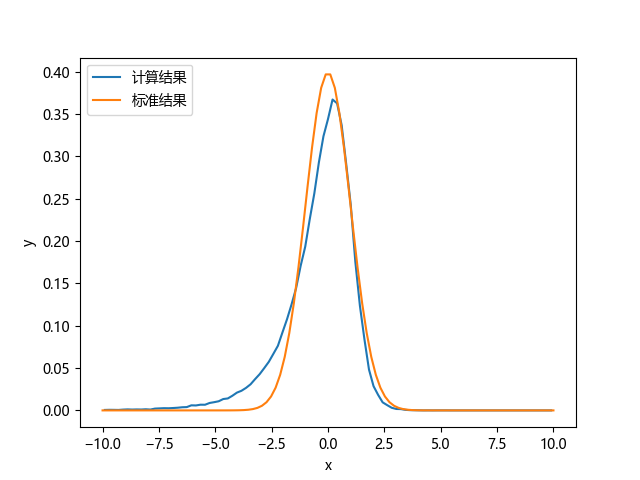
\includegraphics[scale=0.5]{exp_10}}
	\captionsetup{font={small},labelfont=bf}
	\caption{\heiti\zihao{-5}指数分布}
	
\end{figure}
	\begin{figure}[!h]
	\centering
	\subfigure[N=2]{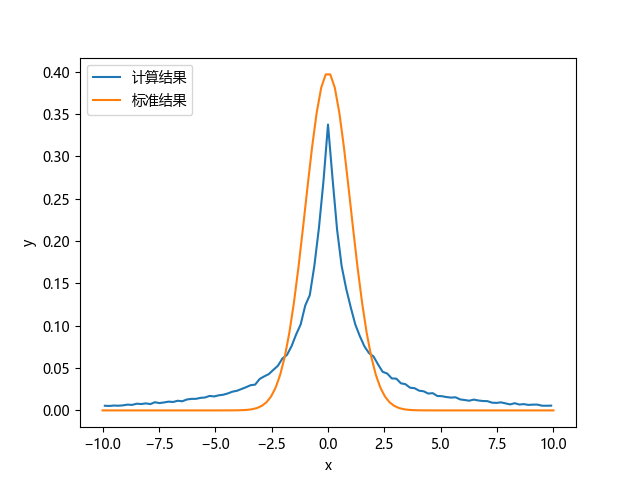
\includegraphics[scale=0.5]{uniform_2}}
	\subfigure[N=5]{	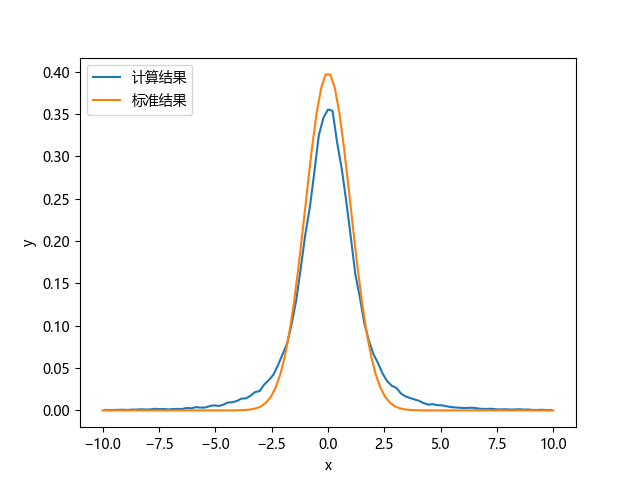
\includegraphics[scale=0.5]{uniform_5}}
	\subfigure[N=10]{	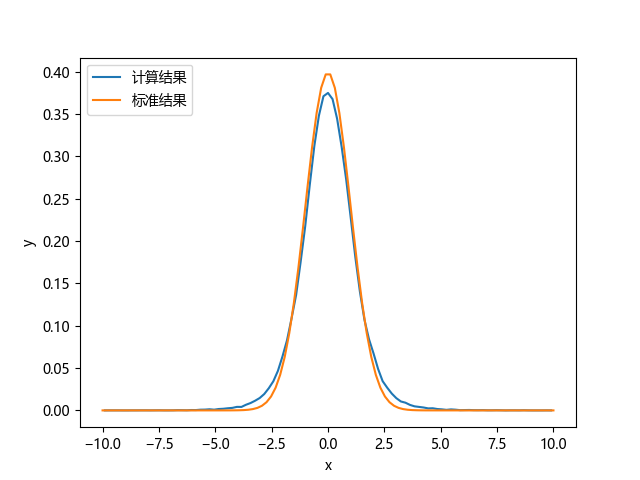
\includegraphics[scale=0.5]{uniform_10}}
	\captionsetup{font={small},labelfont=bf}
	\caption{\heiti\zihao{-5}均匀分布}
	
\end{figure}
\begin{figure}[!h]
	\centering
	\subfigure[N=2]{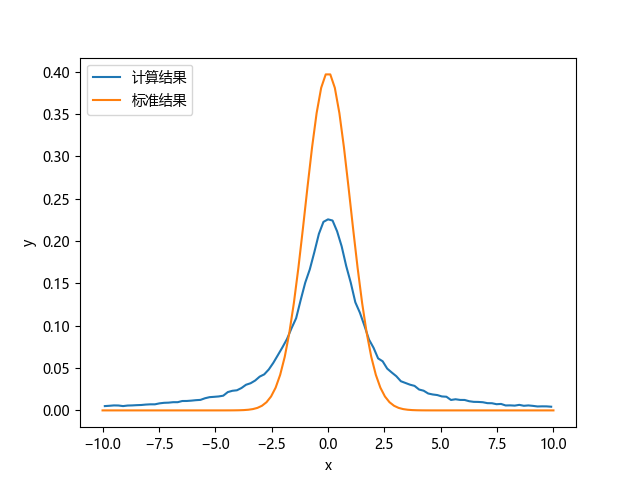
\includegraphics[scale=0.5]{gauss_2}}
	\subfigure[N=5]{	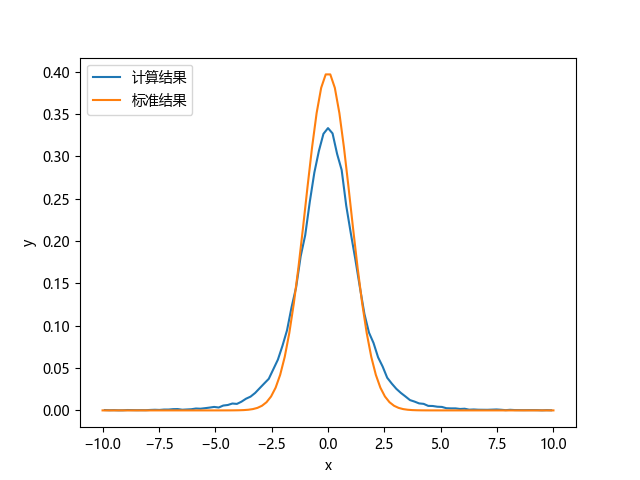
\includegraphics[scale=0.5]{gauss_5}}
	\subfigure[N=10]{	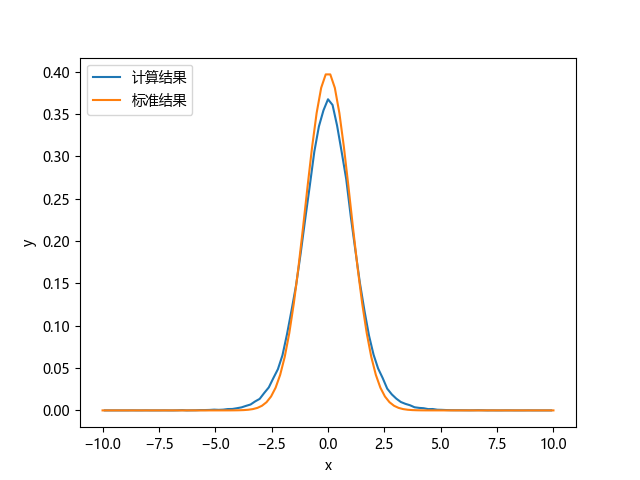
\includegraphics[scale=0.5]{gauss_10}}
	\captionsetup{font={small},labelfont=bf}
	\caption{\heiti\zihao{-5}高斯分布}
	
\end{figure}
	\section{结论}
根据各个分布的误差统计图与标准正态分布图的对比得到,当N=2时,明显与标准正态有较大误差,而且对于泊松分布,由于是离散性分布,且N很小,产生的误差分布也较为离散。由于中心极限定理是在$ N\rightarrow\infty $时误差分布达到的极限为标准正态,可见在N从2到5到10增大时,误差分布曲线逐渐趋近于标准正态分布函数。
\end{document}